\pagebreak
\section{Descrizione Design Pattern}
\label{appendice-pattern}

\subsection{Design Pattern Architetturali}

\subsubsection{MVC}

\textit{Model-View-Controller} (MVC) è un pattern per l'implementazione di interfacce utente. Esso divide un'applicazione software in tre parti interconnesse, in modo da separare nettamente la rappresentazione interna dei dati dal modo in cui essa viene presentata all'utente. Il componente centrale, il modello, consiste di dati business, regole, logica e funzioni. Una \textit{view} può essere qualsiasi output dell'informazione, come ad esempio un testo o un diagramma. Si possono avere molteplici \textit{view} della stessa informazione. La terza parte, il \textit{controller}, si occupa di accettare degli input e di convertirli in \textit{comandi} per il \textit{model} o per la \textit{view}.

Oltre a dividere l'applicazione in queste tre componenti, \glossario{MVC} si occupa anche di definire le interazioni tra esse:

\begin{itemize}

	\item Un \textit{controller} può inviare comandi al \textit{model} per aggiornare il suo stato. Può inoltre inviare comandi alla sua \textit{view} associata, in modo da cambiarne la presentazione;
	\item Un \textit{model} quando cambia il suo stato interno notifica le sue \textit{view} e i suoi \textit{controller} associati. Questo permette alle \textit{view} di cambiare la loro presentazione e ai \textit{controller} di cambiare il loro insieme di comandi disponibili. 
	\item Una \textit{view} viene aggiornata dal \textit{controller} sui dati che necessita per generare un output per l'utente.

\end{itemize}

Sebbene inizialmente sviluppata per applicazioni desktop, \glossario{MVC} è stato usato moltissimo come architettura per le Web application in tutti i principali linguaggi di programmazione. Moltissimi \glossario{framework} commerciali e non sono stati progettati utilizzando questo pattern.

\begin{figure}[H]
\centering 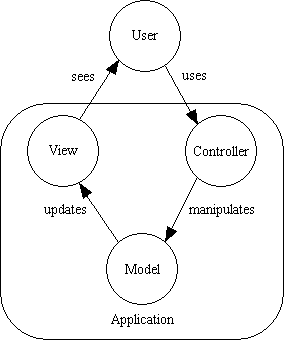
\includegraphics[width=0.4\textwidth]{patterns/mvc.png}
\caption{Struttura logica di Model-View-Controller}
\label{fig:mvc}
\end{figure}

\subsubsection{Middleware} 
Il \glossario{Middleware} è uno strato software che si interpone tra l'applicazione software e il sistema operativo per semplificarne le comunicazioni e la gestione di input/output. Viene solitamente utilizzato in applicazioni distribuite e facilita l'interoperabilità, fornendo servizi che permettono la comunicazione tra applicazioni di sistemi operativi diversi. La distinzione tra lo strato software del sistema operativo è, per alcune entità, arbitraria; può infatti accedere che il \glossario{Middleware} fornisca dei servizi abitualmente attribuibili a un sistema operativo. I primi utilizzi di \glossario{Middleware} risalgono agli anni '80, come soluzione ai problemi di comunicazione tra applicazioni nuove e meno recenti. I servizi \glossario{Middleware} forniscono un set di interfacce che permetto a un'applicazione di:
	
\begin{itemize}

	\item Localizzare facilmente applicazioni o servizi in una rete;
	\item Filtrare dati per renderli \textit{user-friendly} oppure anonimizzarli per renderli pubblicabili, proteggendone la privacy;
	\item Essere indipendente dai servizi di rete;
	\item Essere affidabile e sempre disponibile;
	\item Aggiungere attributi complementari.
	
\end{itemize}
	
Si tratta quindi di funzionalità leggermente più specializzate da quelle normalmente offerte da un sistema operativo. L'avvento del web ha avuto una forte ripercussione sulla diffusione dei software di \glossario{Middleware}. Essi hanno infatti permesso l'accesso sicuro da remoto a database locali. I tipi di \glossario{Middleware} sono:
	
\begin{itemize}
	
	\item \textbf{Message-Oriented Middleware} (\glossario{MOM}): sono \glossario{Middleware} dove le notifiche degli eventi vengono spedite come messaggi tra sistemi o componenti. I messaggi inviati al client vengono memorizzati fintanto che non vengono gestiti, nel frattempo il client può svolgere altro lavoro;
	\item \textbf{Enterprise messaging system}: è un tipo di \glossario{Middleware} che facilita il passaggio di messaggi tra sistemi diversi o componenti in formato standard, spesso utilizzando servizi web o \glossario{XML};
	\item \textbf{Message broker}: è parte dell \emph{entreprise messaging system}. Accoda, duplica, traduce e spedisce messaggi a sistemi o componenti diverse;
	\item \textbf{Enterprise Service Bus}: è definito come qualche tipo di \glossario{Middleware} integrato che supporta sia \glossario{MOM} che dei servizi web;
	\item \textbf{Intelligent Middleware}: gestisce il processamento in tempo reale di grandi volumi di segnali che trasforma in informazioni di business. Particolarmente adatto per architetture scalabili e distribuite;
	\item \textbf{Content-Centric Middleware}: questo tipo di \glossario{Middleware} fornisce una semplice astrazione con la quale le applicazioni possono inoltrare richieste per contenuti univocamente identificati, senza occuparsi su come e dove vanno ottenuti.
		
\end{itemize}	 
	
% possibile add: http://www.networkcomputing.com/netdesign/cdmwdef.htm
\begin{figure}[H]
\centering 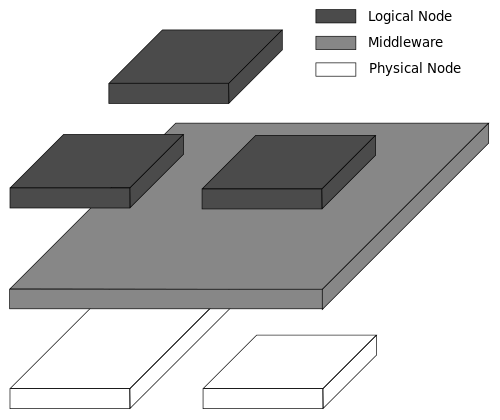
\includegraphics[width=0.7\textwidth]{patterns/Middleware.png}
\caption{Struttura logica di Middleware}
\label{fig:middleware}
\end{figure}

\subsection{Design Pattern Creazionali}

\subsection{Singleton}

Il \glossario{Singleton} è un design pattern creazionale che permette di avere un'unica istanza di una classe con un unico punto di accesso noto. Tale condizione è tipica di alcuni contesti e trova risvolti pratici in svariate applicazioni. Per permettere l'implementazione di questo pattern è sufficiente che la classe stessa si occupi di tracciare la propria istanziazione e bloccarla qualora sia già avvenuta almeno una volta. Il \glossario{Singleton} dovrebbe essere estensibile usando il \emph{subclassing}. Il client può utilizzarne l'estensione senza quindi modificarne il codice.
	
L'utilizzo di questo pattern comporta una serie di conseguenze:

\begin{itemize}

	\item Accesso controllato alla singola istanza: poiché la classe \glossario{Singleton} incapsula la sua unica istanza, è in grado di controllare quando e come i client vi accedono;
	\item Namespace pulito: l'utilizzo di questo pattern risulta migliore rispetto all'uso di variabili globali poiché scongiura l'inquinamento del namespace globale;
	\item Permette raffinamenti di operazioni e rappresentazioni: il \glossario{Singleton} dovrebbe venire sempre esteso prima dell'utilizzo, che in termini pratici si traduce in un operazione banale. Questo può avvenire anche a runtime;
	\item Eventualmente permette un numero variabile di istanze: questo pattern permette, se necessario, di avere istanze multiple mantenendo però il controllo sul numero;
	\item Flessibilità: un modo per avere una funzionalità riconducibile al \glossario{Singleton} è quello di utilizzare le operazioni sulle classi, come per esempio la keyword \code{static} del C++, ma in questo modo è più difficile controllarne il design e permetterne più istanze. Inoltre nel linguaggio succitato le funzioni statiche non sono mai virtuali, rendendone impossibile l'utilizzo polimorfo alle sottoclassi che le ridefiniscono.
	
\end{itemize}

\begin{figure}[H]
\centering 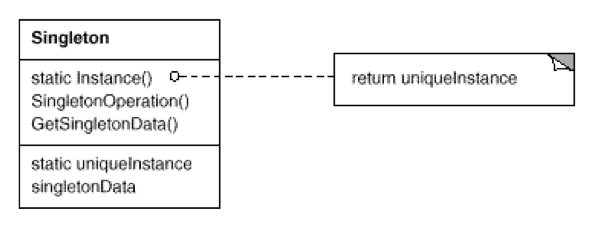
\includegraphics[width=0.7\textwidth]{patterns/Singleton.png}
\caption{Struttura logica di Singleton}
\label{fig:singleton}
\end{figure}

\subsubsection{Registry} %libro dropbox martin fowler

Il \glossario{Registry} è simile ad un oggetto globale che gli altri oggetti usano per accedere a servizi e oggetti comuni. Quando si vuole recuperare un oggetto capita spesso di accedervi tramite un altro oggetto legato da un qualche tipo di associazione, ma in alcuni casi non è possibile conoscere a priori l'oggetto da cui partire, così vi è la necessità di avere un metodo di look-up accedibile tramite il \glossario{Registry}. Le interfacce del \glossario{Registry} possono essere metodi statici.

\begin{figure}[H]
\centering 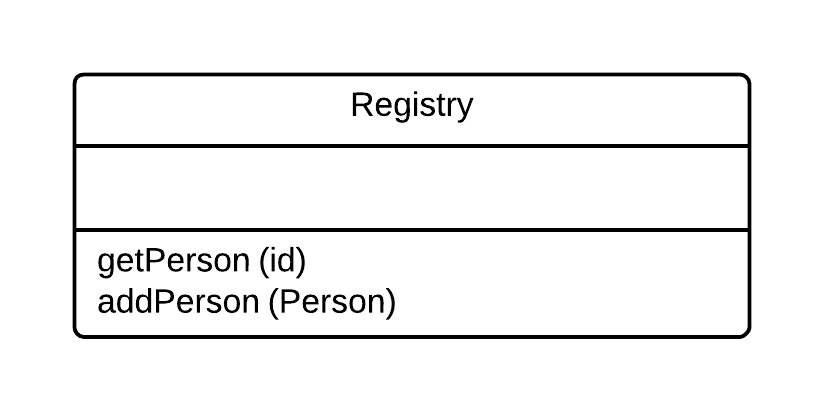
\includegraphics[width=0.6\textwidth]{patterns/registry.png}
\caption{Struttura logica di Registry}
\label{fig:registry}
\end{figure}

\subsubsection{Factory method}
	
Questo pattern definisce un'interfaccia per la creazione di un oggetto, lasciando alle sottoclassi la decisione sulla classe che deve essere istanziata. Consente inoltre di deferire l'istanziazione di una classe alle sottoclassi. Tra i suoi utilizzi ci sono i seguenti casi:

\begin{itemize}

	\item Quando una classe non è in grado di sapere in anticipo le classi degli oggetti che deve creare;
	\item Quando una classe vuole che le sue sottoclassi scelgano gli oggetti da creare;
	\item Quando le classi delegano la responsabilità a una o più classi di supporto e si vuole localizzare in un punto ben preciso la conoscenza di quale o quali classi di supporto vengano delegate.

\end{itemize}

\begin{figure}[H]
\centering 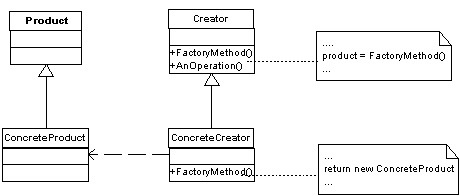
\includegraphics[width=0.8\textwidth]{patterns/factory-method.jpg}
\caption{Struttura logica di Factory Method}
\label{fig:factory-method}
\end{figure}

\subsection{Design Pattern Strutturali}

\subsubsection{Facade}

Questo pattern fornisce un'interfaccia unificata per un insieme di interfacce presenti in un sottosistema. \glossario{Facade} definisce un'interfaccia di alto livello che rende il sottosistema più semplice da utilizzare. Suddividere un sistema in sottosistemi aiuta a ridurne la complessità. Può essere utilizzato nei seguenti casi:

\begin{itemize}

	\item Quando si vuole fornire un'interfaccia semplice a un sottosistema complesso. La complessità dei sottosistemi tende ad aumentare con la loro evoluzione. Molti pattern, quando applicati, portano a un aumento nel numero di classi piccole. Ciò rende il sottosistema maggiormente riusabile e semplice da personalizzare, ma di utilizzo più difficile per i client che non richiedono alcuna personalizzazione. Un \textit{facade} può fornire una vista semplice di base su un sottosistema che si rivela essere sufficiente per la maggior parte dei client. Soltanto i client che richiedono una personalizzazione maggiore dovranno guardare dietro la facciata;
	\item Nei casi in cui sono molte le dipendenze fra i client e le classi che implementano un'astrazione. Introducendo un \textit{facade} si disaccoppia il sottosistema dai client e dagli altri sottosistemi, promuovendo quindi la portabilità e l'indipendenza di sottosistemi;
	\item Quando si vogliono organizzare i sottosistemi in una struttura a livelli. Un \textit{facade} può essere utilizzato per definire un punto di ingresso ad ogni livello. Nel caso in cui i sottosistemi non siano indipendenti e le dipendenze esistenti possano essere semplificate facendo comunicare tra loro i sottosistemi soltanto attraverso i rispettivi oggetti \textit{facade}.

\end{itemize}

\begin{figure}[H]
\centering 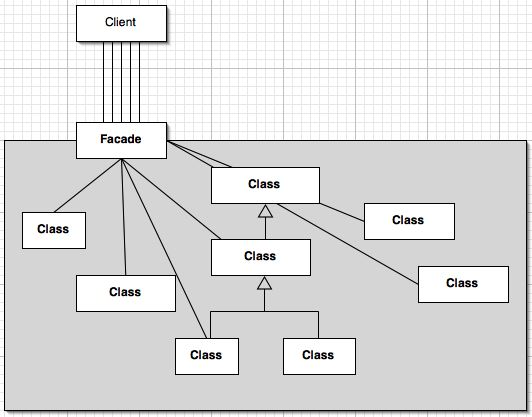
\includegraphics[width=0.7\textwidth]{patterns/facade.jpg}
\caption{Struttura logica di Facade}
\label{fig:facade}
\end{figure}

\subsection{Design Pattern Comportamentali}

\subsubsection{Chain of Responsibility}
Il \glossario{Chain of Responsibility} è un pattern comportamentale che permette di separare i \emph{sender} dai \emph{receiver} delle richieste. La richiesta attraversa una catena di oggetti per essere intercettata solo quando raggiunge il proprio gestore. Viene utilizzato quando non è possibile determinare staticamente il \emph{receiver} oppure l'insieme di oggetti gestori cambia dinamicamente a runtime.
Le richieste vengono dette \emph{implicite} poiché il \emph{sender} non ha alcuna conoscenza sull'identità del ricevente. Per permettere alla richiesta di attraversare la catena e per rimanere \emph{implicita}, ogni \emph{receiver} condivide un interfaccia comune per gestire le richieste ed accedere al proprio successore. 
La gerarchia che vorrà inviare richieste dovrà avere una superclasse che dichiara un metodo \emph{handler} generico. La specializzazione di tale metodo avviene tramite \emph{overriding} nelle sottoclassi opportune, come illustrato in figura \ref{fig:chainofresponsibility}.	

L'utilizzo di questo pattern comporta una serie di conseguenze:
		
\begin{itemize}

	\item Ridotto accoppiamento: gli oggetti non sono a conoscenza di chi gestirà la richiesta ma sanno solo che verrà gestita in modo appropriato. Inoltre non bisognerà manutenere i riferimenti a tutti i possibili riceventi;
	\item Aggiunge flessibilità nell'assegnamento delle responsabilità degli oggetti: è possible distribuire le responsabilità tra gli oggetti a runtime modificandone la gerarchia. Staticamente è possibile usare il \emph{subclassing} per specializzare i gestori;
 	\item Non c'è garanzia che la \emph{request} venga gestita, questo può avvenire quando la catena non è stata costruita in modo rigoroso.
 	
\end{itemize}
	 	
\begin{figure}[H]
\centering 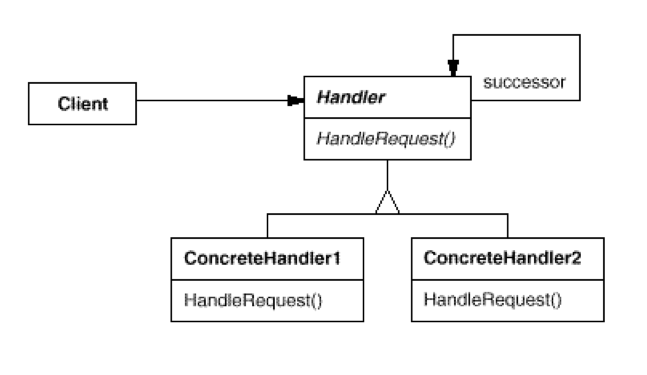
\includegraphics[width=0.7\textwidth]{patterns/ChainOfResponsability.png}
\caption{Struttura del Chain of Responsibility}
\label{fig:chainofresponsibility}
\end{figure}
	
\subsubsection{Strategy}

\textit{Strategy} ha come scopo quello di definire una famiglia di algoritmi, incapsularli e renderli intercambiabili. Permette agli algoritmi di variare indipendentemente dal client che ne fa uso. È opportuno usare il pattern \textit{strategy} nei seguenti casi:

\begin{itemize}

	\item Molte classi correlate differiscono fra loro solo per il comportamento. \textit{Strategy} fornisce un modo per configurare una classe con un comportamento scelto fra tanti;
	\item Sono necessarie più varianti di un algoritmo. Per esempio, è possibile definire più algoritmi con bilanciamenti diversi fra occupazione in memoria, velocità di esecuzione, ecc. Possiamo usare il pattern \textit{Strategy} quando queste varianti sono implementate sotto forma di gerarchia di classi di algoritmi;
	\item Un algoritmo usa una struttura dati che non dovrebbe essere resa nota ai client. Il pattern \textit{strategy} può essere usato per evitare di esporre strutture dati complesse e specifiche dell'algoritmo;
	\item Una classe definisce molti comportamenti che compaiono all'interno di scelte condizionali multiple. Al posto di molte scelte condizionali si suggerisce di spostare i blocchi di codice correlati in una classe \texttt{Strategy} dedicata.
	
\end{itemize}

\begin{figure}[H]
\centering 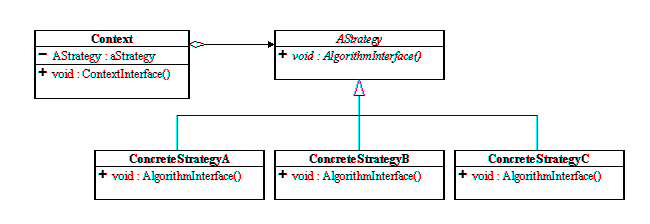
\includegraphics[width=0.9\textwidth]{patterns/strategy.jpg}
\caption{Struttura logica di Strategy}
\label{fig:strategy}
\end{figure}
	
\subsubsection{Dependency Injection}

Il \glossario{Dependency Injection} è un \glossario{Design Pattern} che permette la separazione del comportamento degli oggetti dalla loro dipendenze. Invece di istanziare le classi in modo diretto ogni componente riceve i riferimenti agli altri componenti necessari come parametri nel costruttore. Un utilizzo comune è quello con i 	\emph{plugin} che vengono caricati dinamicamente. Gli elementi coinvolti sono:
	
\begin{itemize}
	\item Un dipendente consumatore;
	\item Una dichiarazione delle dipendenze tra la componenti, definita come contratto di un interfaccia;
	\item Un injector che crea istanze di classi che implementano una data dipendenza su richiesta.

\end{itemize}

Il \textit{dependent object} dichiara da quali componenti dipende. L'\textit{injector} decide quali classi soddisfano suoi requisiti e in caso affermativo gliele fornisce. Questa operazione può avvenire anche a runtime. Questo è un chiaro vantaggio poiché possono essere create dinamicamente diverse implementazioni di un componente software da passare allo stesso test. In questo modo il test può testare componenti diverse senza sapere che le loro implementazioni sono diverse.
Lo scopo principale di questo pattern è quello di permettere una selezione a runtime su più implementazioni di una interfaccia dipendente. È particolarmente utile per fornire delle implementazioni di \glossario{stub} per componenti complesse, ma anche per gestire i plugin e per inizializzare servizi software. I test di unità comportano delle problematiche, poiché spesso richiedono la presenza di una parte di infrastruttura non ancora implementata. Il \glossario{Dependency Injection} semplifica il processo di testing per un istanza isolata. Poiché le componenti dichiarano le proprie dipendenze, un test può automaticamente istanziare le componenti necessarie.
	 
L'utilizzo di questo pattern comporta una serie di conseguenze:

\begin{itemize}

	\item Vi è una riduzione di \glossario{Boilerplate code} poiché il lavoro di set up delle dipendenze viene gestito da un componente dedicato;
	\item Offre una certa flessibilità di configurazione perché diverse implementazione di un servizio posso essere usate senza essere ricompilate;
	\item Facilita la scrittura di codice testabile;
	\item Le dipendenze dichiarate sono \glossario{black box}, questo rende più difficile trovare gli errori al loro interno;
	\item Le dipendenze non completamente implementate o errate generano errori a runtime e non a tempo di compilazione;
	\item Rende il codice più difficile da manutenere;
	\item L'\textit{injection} a runtime di dipendenze va ad inficiare le prestazioni;
	\item I benefici sono difficilmente commisurabili rispetto ai costi di implementazione.

\end{itemize}
		
Di seguito vengono elencati tre modi con cui un oggetto può ricevere un riferimento da un modulo esterno:

\begin{itemize}

	\item \textbf{Interface injection}: l'oggetto fornisce un interfaccia che gli utenti possono implementare in modo da ottenere a runtime le dipendenze;
	\item \textbf{Setter injection}: il \textit{dependent module} espone un metodo \textit{setter} che il \glossario{framework} usa per iniettarvi le dipendenze;
	\item \textbf{Constructor injection}: le dipendenze vengono fornite tramite il costruttore della classe.

\end{itemize}

\begin{figure}[H]
\centering 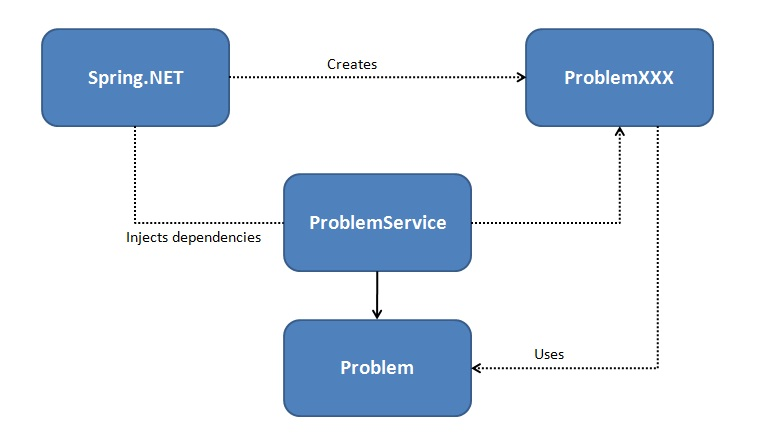
\includegraphics[width=0.7\textwidth]{patterns/dependency-injection.jpg}
\caption{Struttura logica di Dependency Injection}
\label{fig:strategy}
\end{figure}


\subsubsection{Command}

Il command pattern è uno dei \glossario{Design Pattern} che permette di isolare la porzione di codice che effettua un'azione (eventualmente molto complessa) dal codice che ne richiede l'esecuzione. L'azione è incapsulata nell'oggetto \textit{Command}. L'obiettivo è rendere variabile l'azione del \textit{client} senza però conoscere i dettagli dell'operazione stessa. Altro aspetto importante è che il destinatario della richiesta può non essere deciso staticamente all'atto dell'istanziazione del \textit{Command} ma dev'essere ricavato a tempo di esecuzione. È possibile incapsulare un'azione in modo che questa sia atomica. È così possibile implementare un paradigma basato su transazioni in cui un insieme di operazioni è svolto in toto o per nulla.

\begin{figure}[H]
\centering 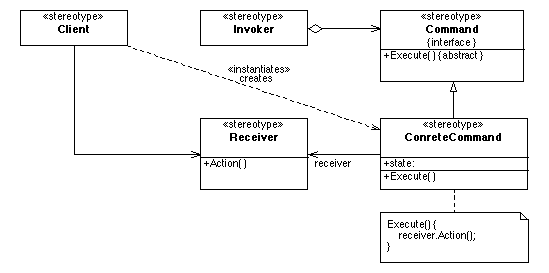
\includegraphics[width=\textwidth]{patterns/command.png}
\caption{Struttura logica di Command}
\label{fig:strategy}
\end{figure}
